\section{Desired model}

\subsection{Resources of Data center}
To simplify the model of a data center we will not consider CPU, memory, storage and intra data center network separately.
Instead, in this paper, we will use an abstraction of one dimensional computational resource.

Hosting VMs in a data center can be modeled in two ways: with or without competition for computational resource.

In the first approach, the resources of a data center are aggregated in one pool that is continuously divisible.
%Each VM gets an equal part of available resources inversely proportional to the number of VMs hosted in the data center.
%The bigger is the number of VMs hosted in the data center, the smaller amount of resources each of them gets.
The pool of resources is divided evenly among all VMs.
Hence, when the number of VMs hosted in the data center increases, the amount of resources available for each VM shrinks.
Consequently the service time of processing requests of each VM lengthens.

In the second approach, the resources of a data center are discrete and each computational unit is used exclusively by one VM.
Therefore, there is no influence of one VM on another.
To incorporate the fact that the amount of resources is finite we put a limit on the maximal number of VMs that can be hosted in one data center.

\subsection{Overhead of VM Migration}
The overhead of VM migration can be also modeled in different ways depending on the manner how data center resources are represented.

When using the approch where VMs are competing for computational resources, the overhead of VM migration can be modeled by running two instances of VM on both source and destination DC during the time of migration. 

\begin{figure}[tb]
	\centering
	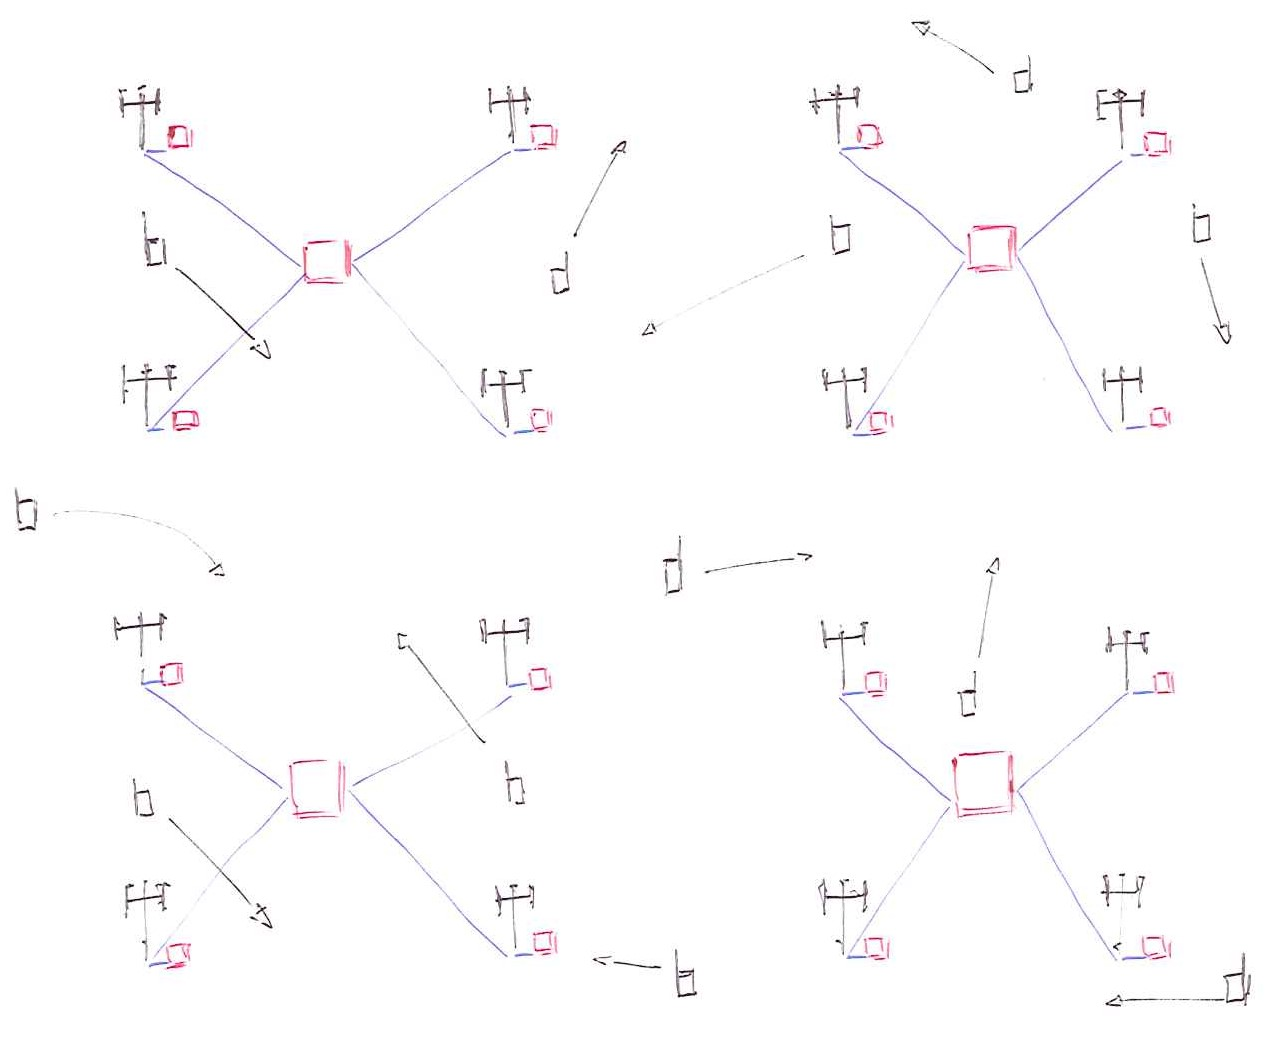
\includegraphics[width=\linewidth]{performance_delay.jpg} 
	\caption{Performance model}
	\label{fig:performance_model}
\end{figure}

As the the topology of the \xcloud and future mobile networks is yet to be determined, and due to the fact that we want to research the effects of mobility without a socio-economic model, the network 